% ---------------------------------------------------------------- Method validation: closed loop
\subsection*{Closed-loop control of live training}
Offline replay cannot show what a learning-rate change does. We therefore let the complete controller (feature extraction, supervisor, gate, executor) control live training processes. For each workload we re-ran the 12 configurations of seed 2 under control, with the gate trained on the \emph{other three} workloads, and compared each controlled run with its uncontrolled recording, which has the same seed and settings. Control is asynchronous, as in deployment: the process keeps training while the controller decides, and a learning-rate change takes effect at the next epoch boundary. Until the first intervention, every controlled run reproduced its uncontrolled curve, which confirms that the comparison is paired.

\begin{table}[t]
\centering
\caption{Closed-loop control of live training (12 configurations of seed 2 per row). Top: gates trained on the other three workloads, with the learning-rate guard. Bottom: effect of the guard. ``Change'' is the relative change in best validation loss against the same run uncontrolled (negative is better); ``worse'' counts runs more than 2\% worse; $p$ is the Wilcoxon signed-rank test of controlled against uncontrolled best validation loss; the last column gives learning-rate halvings in total and (in brackets) the most in one run.}
\label{tab:closed}
\footnotesize
\setlength{\tabcolsep}{3.5pt}
\resizebox{\textwidth}{!}{%
\begin{tabular}{lrrrrrrrr}
\toprule
Workload / condition & Runs & Epochs used & Saved (\%) & Median change (\%) & Min / max (\%) & Worse & $p$ & LR halvings \\
\midrule
\multicolumn{9}{l}{\emph{Unseen-workload gate, guard on}}\\
\tabinput{generated/table_closed_lowo.tex}
\midrule
\multicolumn{9}{l}{\emph{Learning-rate guard off versus on}}\\
\tabinput{generated/table_closed_guard.tex}
\bottomrule
\end{tabular}}
\end{table}

\begin{figure}[t]
\centering
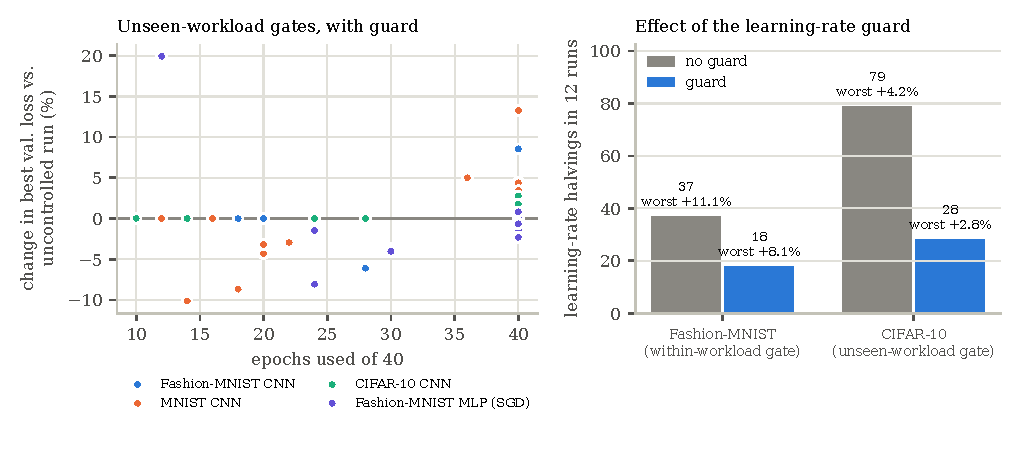
\includegraphics[width=\textwidth]{figures/closed_loop.pdf}
\caption{Closed-loop control. Left: for each of the 48 live runs controlled by a gate that had never seen its workload, epochs used and the change in best validation loss against the same run uncontrolled. Right: learning-rate halvings over 12 runs without and with the guard, and the worst single-run change in best validation loss.}
\label{fig:closed}
\end{figure}

\paragraph{Unseen workloads} Over all 48 runs the controller used \C{lowoall}{used} of \C{lowoall}{budget} epochs (\C{lowoall}{saved}\% saved) and stopped \C{lowoall}{stopped} runs early (Table~\ref{tab:closed}, Fig.~\ref{fig:closed}). The best validation loss was unchanged in the median (\C{lowoall}{relmed}\%) and not significantly different from uncontrolled training ($p\C{lowoall}{p}$); \C{lowoall}{better} runs ended more than 2\% better and \C{lowoall}{worse} more than 2\% worse, and the mean change in validation accuracy at the best checkpoint was $\C{lowoall}{acc}$ percentage points. Savings were lower than in offline replay of the same 48 configurations (\X{offlineSeedTwoSaved}\%) because a run's curve changes after a learning-rate halving, so the controlled runs are no longer the recorded ones, and because a stop decided asynchronously takes effect only at the process's next epoch boundary. The largest loss, \C{lowomlpsgd}{relmax}\%, is the unstable SGD run discussed above, which the gate stopped before its isolated late minimum.

\paragraph{The learning-rate guard} Without the guard the executor halved the learning rate up to \C{fmnistnoguard}{adjmax} times in one Fashion-MNIST run and up to \C{cifarnoguard}{adjmax} times in one CIFAR-10 run, leaving those runs at a small fraction of their initial learning rate. With the guard, at most \C{fmnistguard}{adjmax} halvings per run were executed (\C{fmnistguard}{deferred} further requests were deferred on Fashion-MNIST), and the worst single-run change in best validation loss fell from $+\C{fmnistnoguard}{relmax}\%$ to $+\C{fmnistguard}{relmax}\%$ on Fashion-MNIST and from $+\C{cifarnoguard}{relmax}\%$ to $+\C{lowocifar}{relmax}\%$ on CIFAR-10, at the cost of fewer epochs saved on Fashion-MNIST (\C{fmnistguard}{saved}\% against \C{fmnistnoguard}{saved}\%). Neither condition changed best validation loss significantly. The guard is a deployment safeguard rather than a learned component, and its two parameters (spacing and maximum count) should be revisited for jobs with very different schedules.
